%!TEX root = ../../main.tex
\section{Results}
\label{sec:Results}

\subsection{Experiment 1}
\label{sub:Experiment 1 - Results}
Figure~\ref{fig:Main radioprotectant plot - Rebecca data} shows the results of the logistic curve fits to the fidelity data plotted in Figure~\ref{fig:Rebecca data}. The five-pointed stars are the points where the fitted logistic curves reach a fidelity value of 0.71. This value was chosen because all samples reached that value. The six-pointed stars are the maximum curvature points of the fitted logistic curves. To compare the efficacies of each radioprotectant compound, the dose at which these points occur are plotted for each scavenger in Figure~\ref{fig:Combined Scavenger results - Rebecca data}.

\begin{figure}
    \centering
    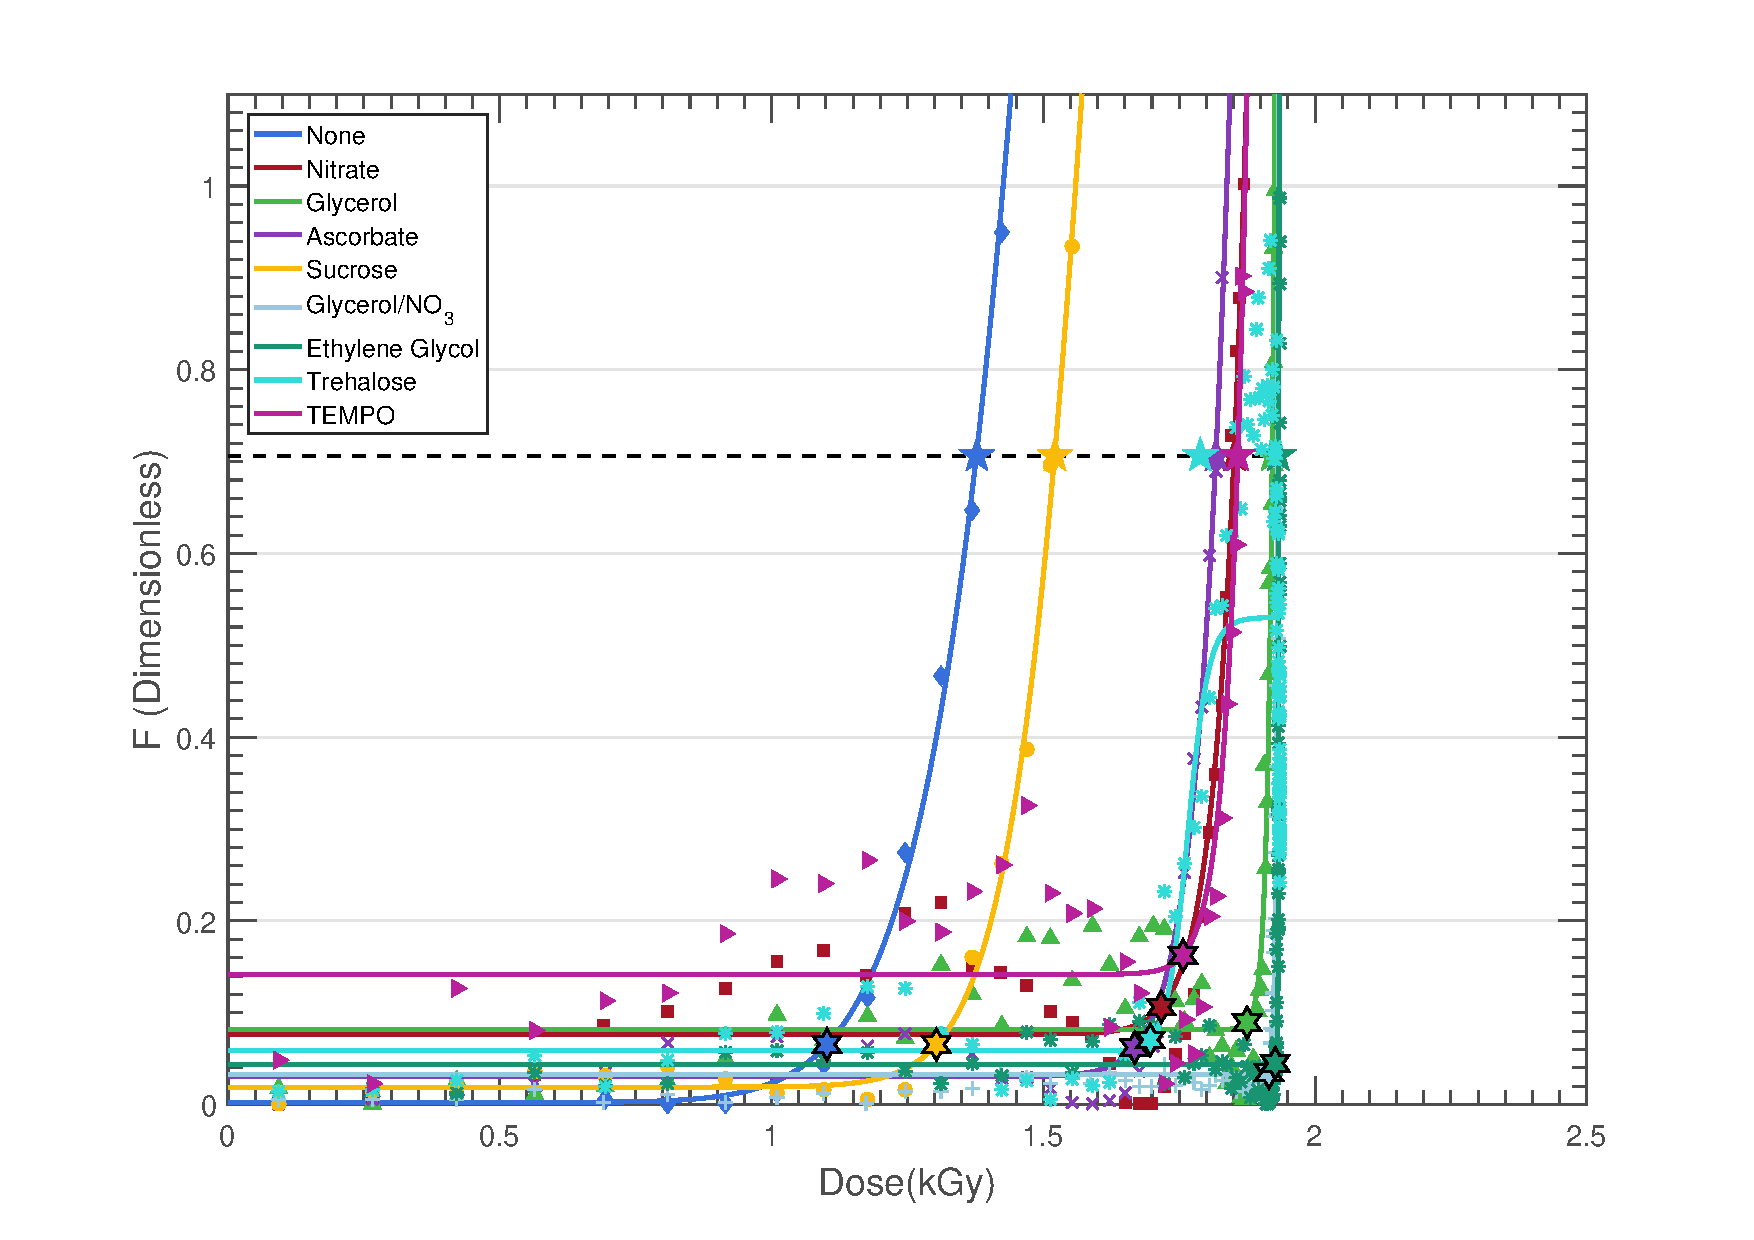
\includegraphics[width=0.8\textwidth]{figures/saxs/ScavengerPlot.pdf}
    \caption{Fidelity values against dose for each radioprotectant along with their corresponding fitted logistic curves. The five-pointed stars represent the points where the fitted logistic curves reach a fidelity value of 0.71. The six-pointed stars are the maximum curvature points of the fitted curves.}
    \label{fig:Main radioprotectant plot - Rebecca data}
\end{figure}

Figure~\ref{fig:Scavenger plot - arbitrary fidelity value} shows the dose taken to reach a fidelity value of 0.71 for each scavenger. This plot shows that etheylene glycol is the most effective radioprotectant at $5\ mM$ concentration, closely followed by the glycerol/sodium nitrate mixture and then glycerol alone. It is clear from these results that adding a radioprotectant allows useable data to be collected for longer because the sample is less sensitive to irradiation.

Similar conclusions are obtained from Figure~\ref{fig:Scavenger plot - maximum curvature} where the dose at which maximum curvature is reached is plotted for each radioprotectant. Again etheylene glycol is shown to be the most effective radioprotectant at $5\ mM$ concentration, followed by the glycerol/sodium nitrate mixture and then glycerol alone. The only difference in the ordering of the relative efficacies of the radioprotectants between the two plots is that trehalose is more effective than ascorbate when using the maximum curvature metric, whereas the opposite is true when using the time to reach a fidelity of 0.71 metric.
\begin{figure}
    \centering
    \begin{subfigure}[b]{0.8\textwidth}
            \centering
            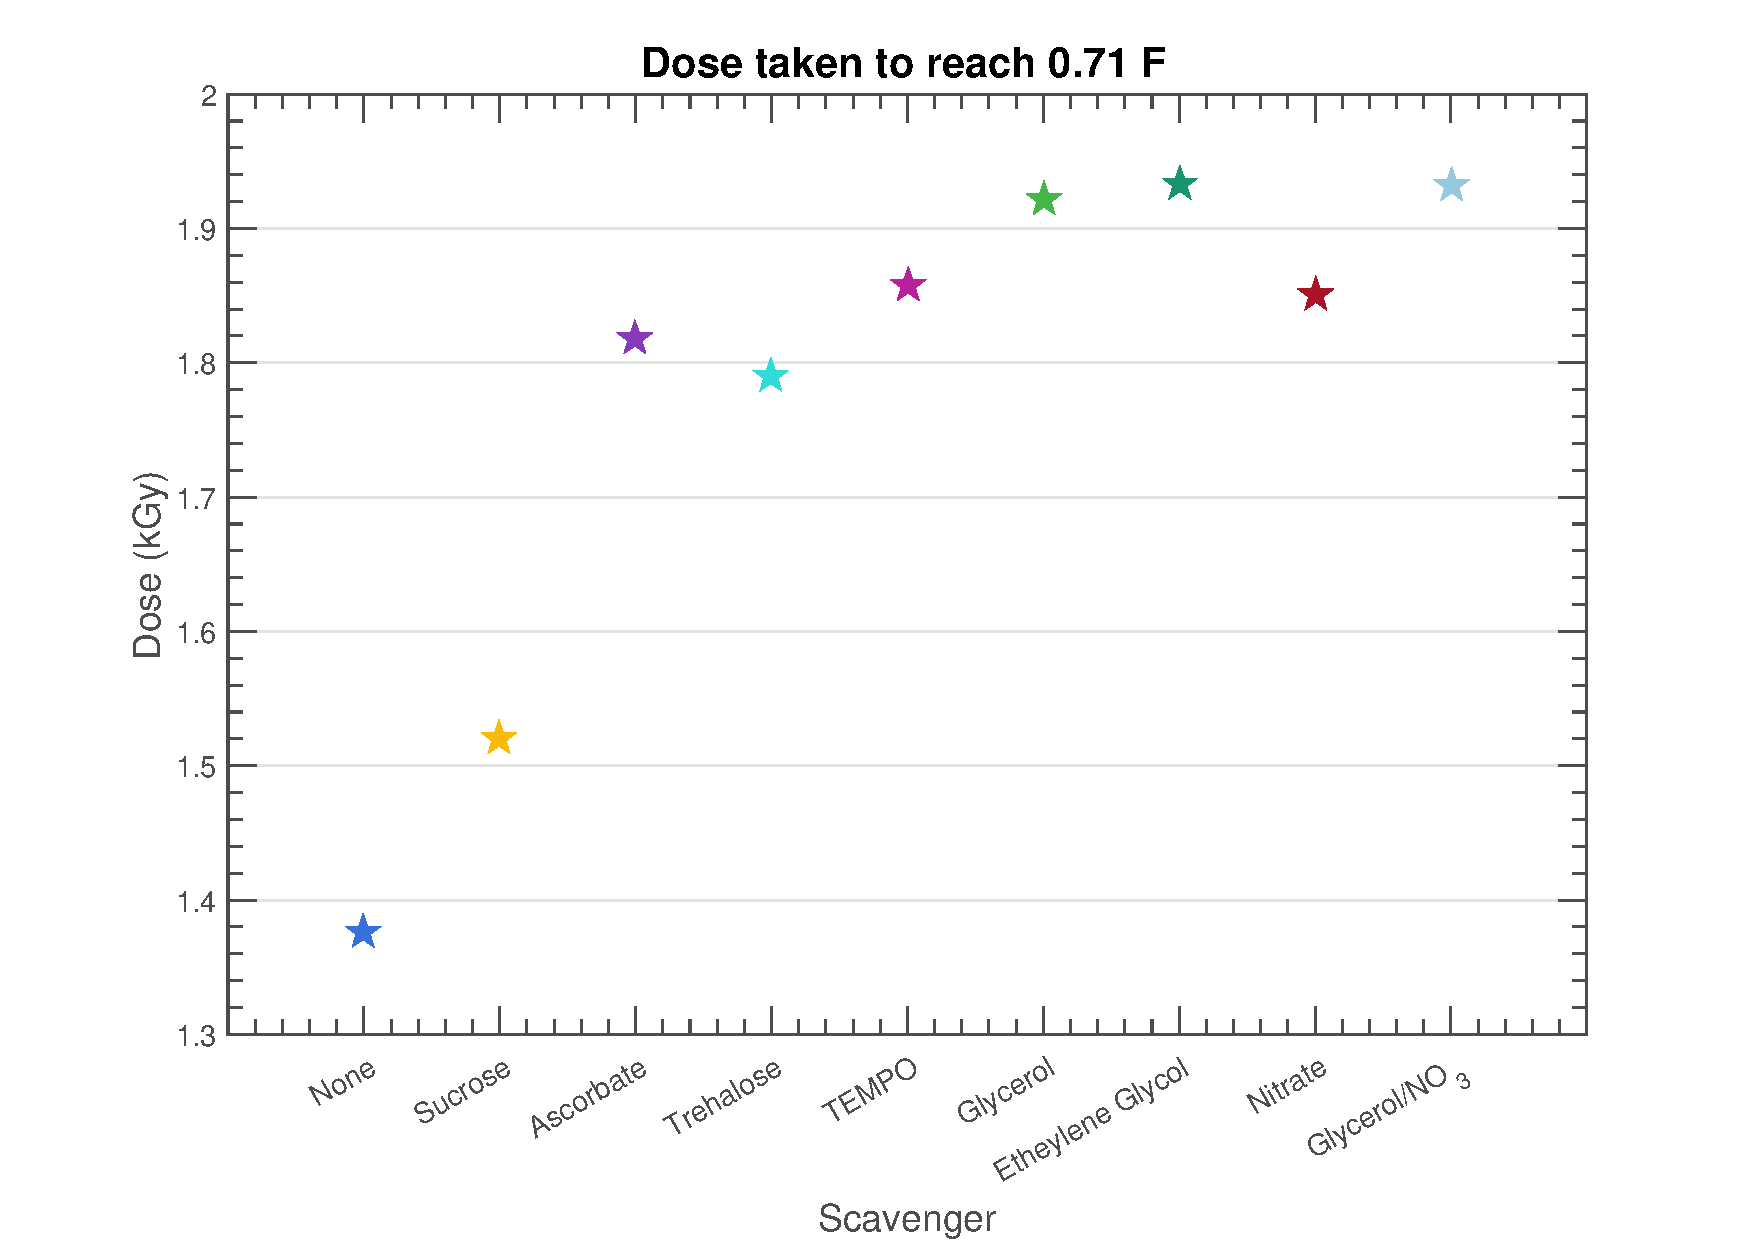
\includegraphics[width=\textwidth]{figures/saxs/ScavengerComparisonPlot.pdf}
            \caption{Dose taken to reach a fidelity value of 0.71 for each scavenger.}
            \label{fig:Scavenger plot - arbitrary fidelity value}
    \end{subfigure}
    \\
    \begin{subfigure}[b]{0.8\textwidth}
            \centering
            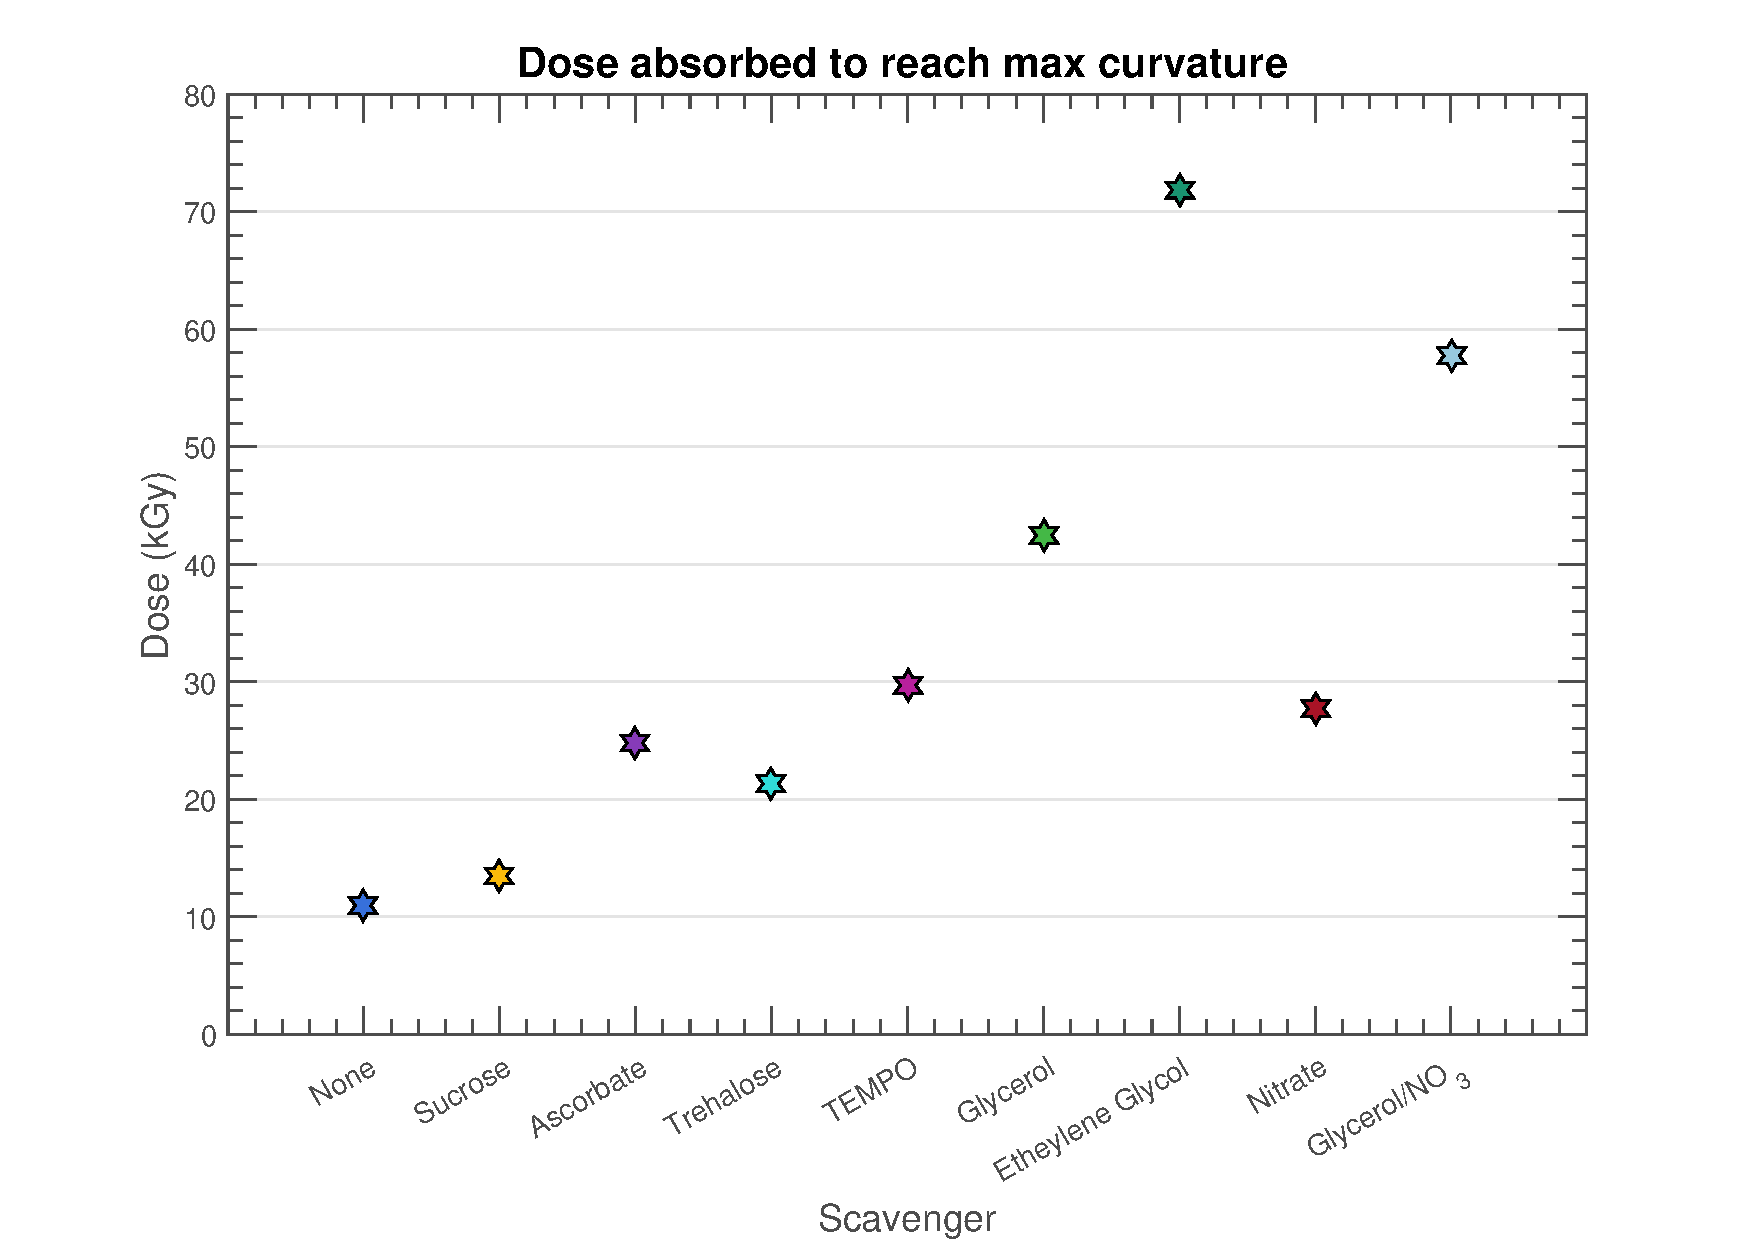
\includegraphics[width=\textwidth]{figures/saxs/ScavengerCurvatureComparisonPlot.pdf}
            \caption{Dose at which maximum curvature is reached}
            \label{fig:Scavenger plot - maximum curvature}
    \end{subfigure}
    \caption{}
    \label{fig:Combined Scavenger results - Rebecca data}
\end{figure}

\subsection{Experiment 2}
\label{sub:Experiment 2 - Results}

\subsubsection{Comparing radiation damage onset metrics}
\label{subs:Comparing radiation damage onset metrics}
In section \ref{sub:Data analysis - experiment 2} a metric for assessing the frame at which radiation damage had become significant was presented based on the CorMap test.
Namely this metric was defined at the point when three consecutive frames were defined as dissimilar ($m = 3$) resulting from the CorMap test with threshold $\alpha = 0.01$.
However an automatic data analysis pipeline is also run at beamline BM29 during data collection \cite{brennich2016online}, which is integrated into the beamline control system, \textit{BsxCuBE}.
Merging analysis of frames is a performed as part of the pipeline and hence there are also thresholds for radiation damage onset according to this analysis.
The metric described in section \ref{sub:Data analysis - experiment 2} will be referred to as the textcolor{red}{\textit{CorMap}} metric whereas the metric used as part of the automatic pipeline analysis will be referred to as the \textit{BsxCuBE} metric.

Figure~\ref{fig:SAXS Metric comparison} shows how the two metrics compare for each compound at all concentrations.
Generally the two metrics agree on the order of the efficacy of the various radioprotectant compounds but the \textit{BsxCuBE} metric always suggests that more frames can be merged then the \textit{Cormap} metric.
Given that the \textit{Cormap} metric was designed not to flag single dissimilar frames as an overall merging threshold, this result is quite surprising.
It suggests that the \textit{BsxCuBE} metric employs a very different method to assess the similarity of frames than the \textit{Cormap} metric.
\textcolor{red}{
    \begin{myenumerate}
        \item \hypertarget{todo:Ask Adam about BsxCuBE}{\textbf{TODO:} ask adam about the BsxCuBE metric.}
        The paper suggest that it too uses the CorMap method with the same $\alpha = 0.01$ but the results don't match up.
    \end{myenumerate}
}
\begin{figure}
    \centering
    \begin{subfigure}[b]{0.45\textwidth}
            \centering
            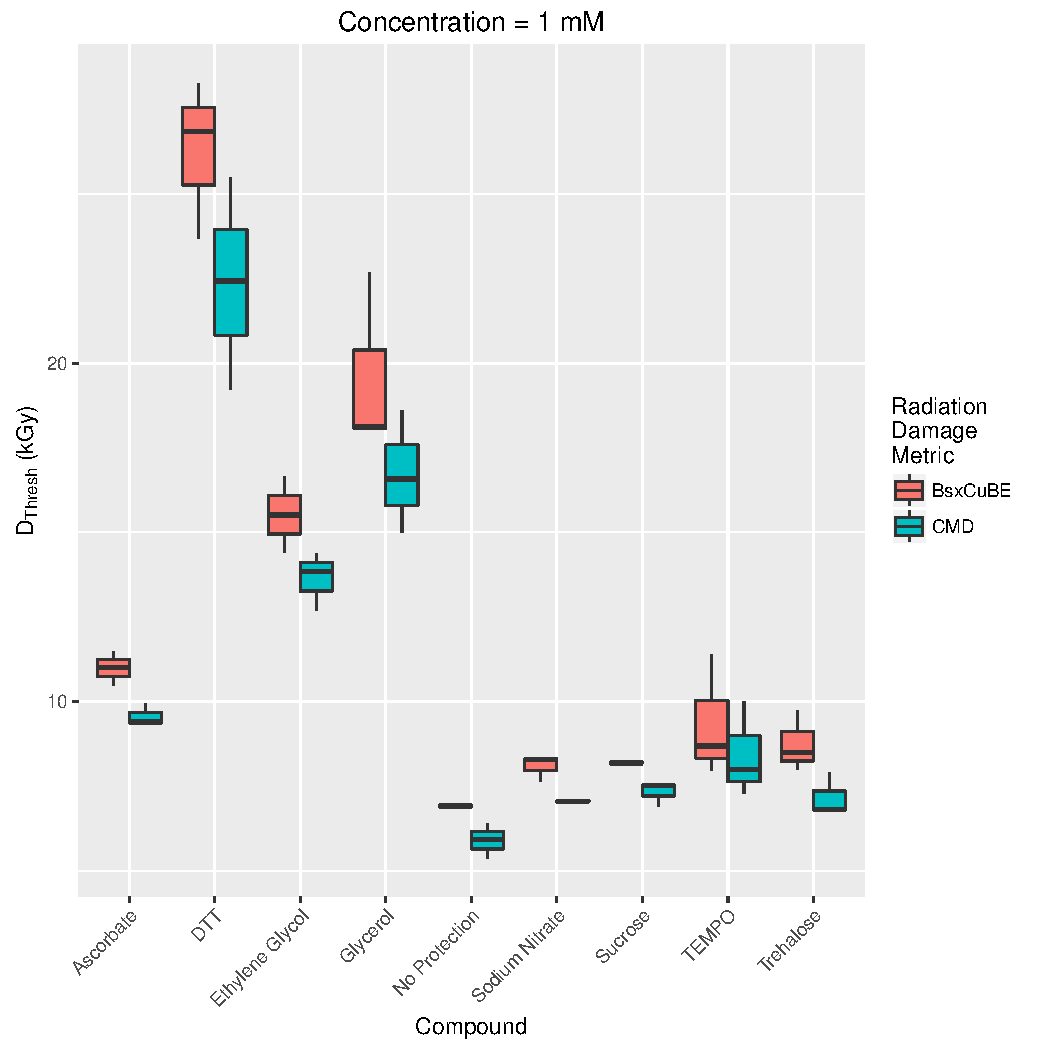
\includegraphics[width=\textwidth]{figures/saxs/Conc_1_dose.pdf}
            \caption{}
            \label{fig:SAXS Metric comparison - 1mM}
    \end{subfigure}
    \qquad
    \begin{subfigure}[b]{0.45\textwidth}
            \centering
            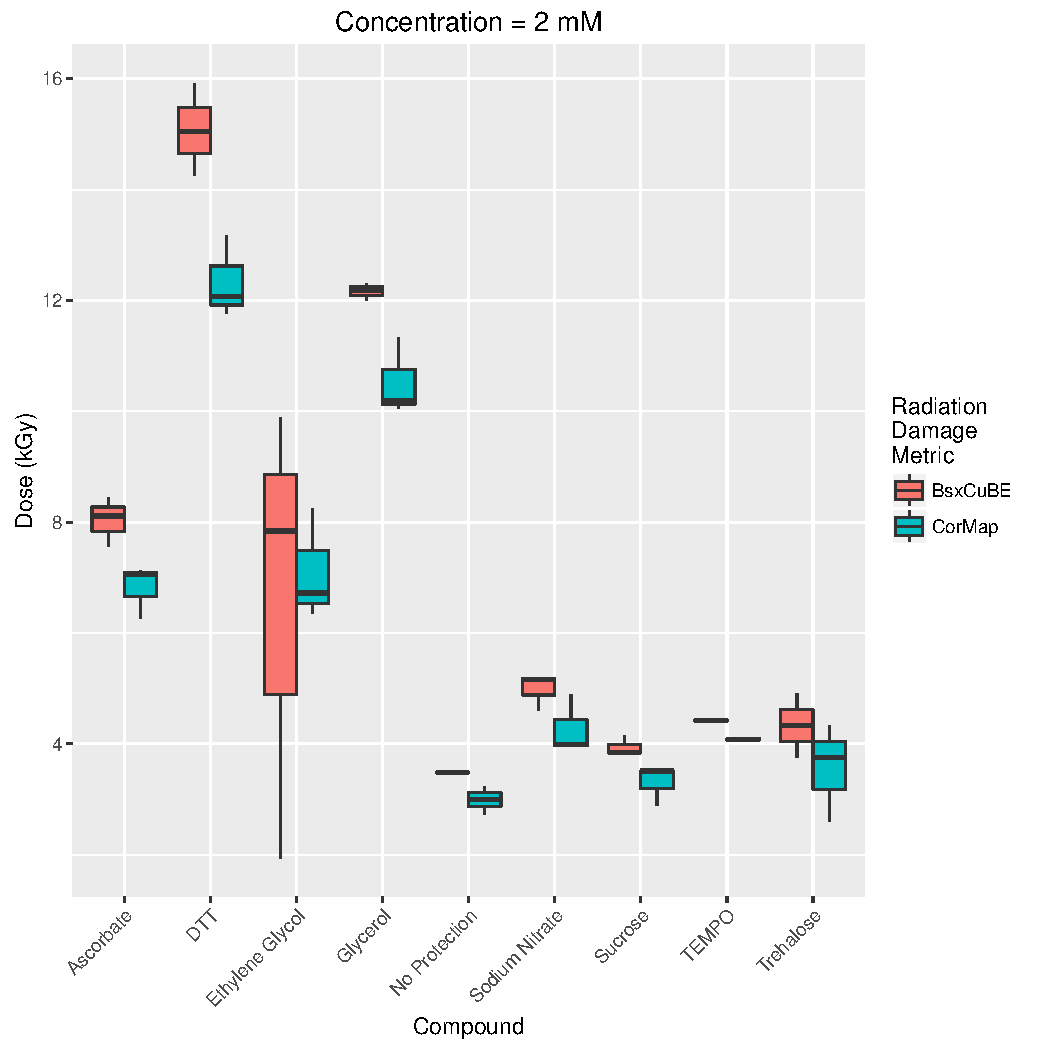
\includegraphics[width=\textwidth]{figures/saxs/Conc_2_dose.pdf}
            \caption{}
            \label{fig:SAXS Metric comparison - 2mM}
    \end{subfigure}
    \\
    \begin{subfigure}[b]{0.45\textwidth}
            \centering
            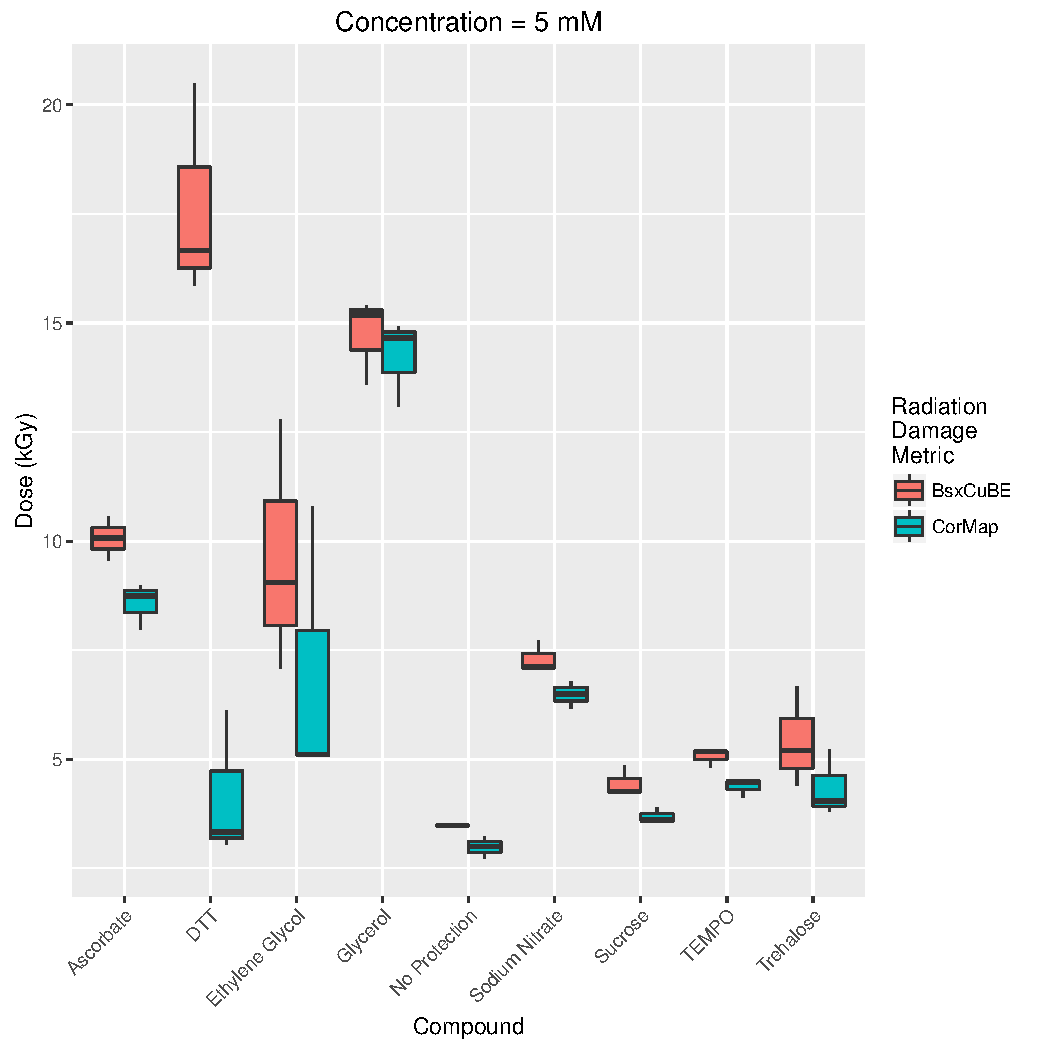
\includegraphics[width=\textwidth]{figures/saxs/Conc_5_dose.pdf}
            \caption{}
            \label{fig:SAXS Metric comparison - 5mM}
    \end{subfigure}
    \qquad
    \begin{subfigure}[b]{0.45\textwidth}
            \centering
            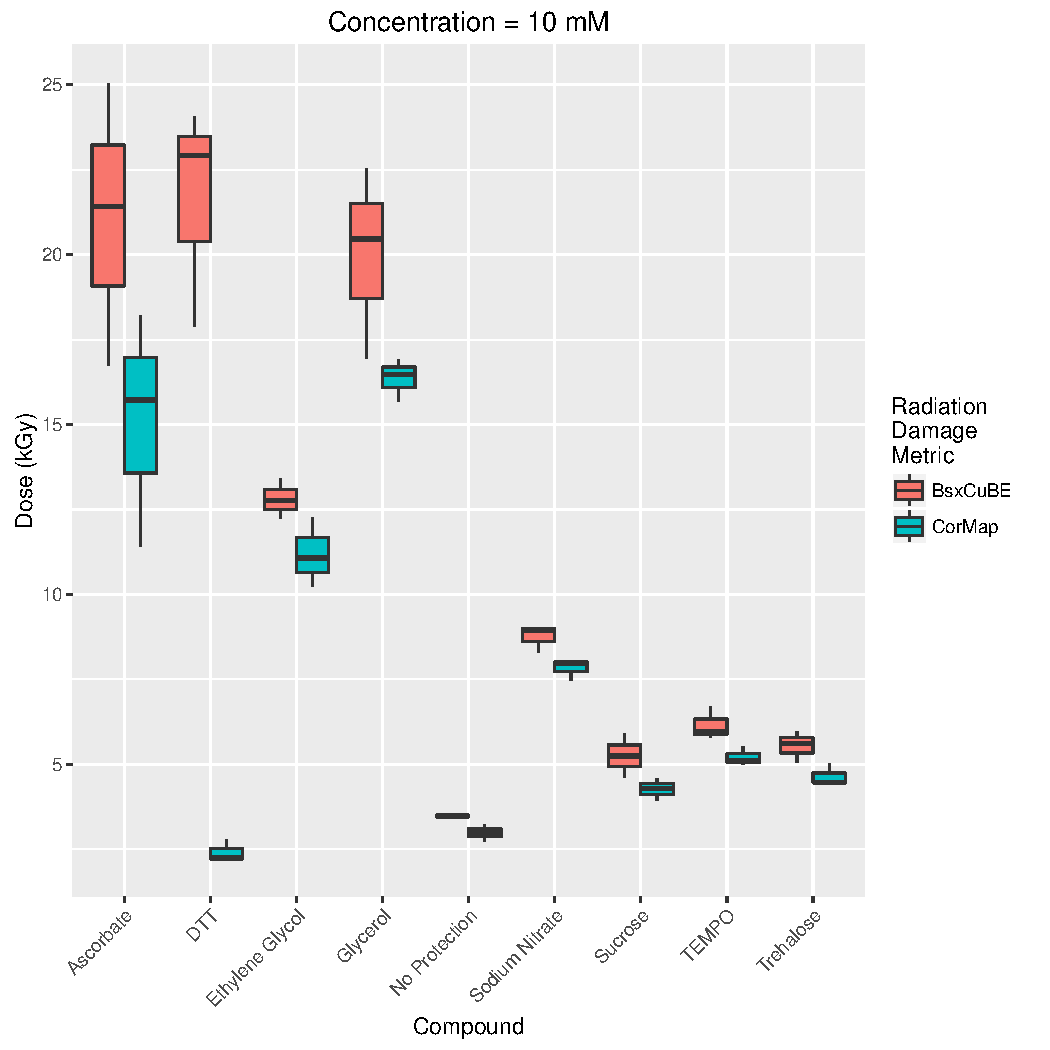
\includegraphics[width=\textwidth]{figures/saxs/Conc_10_dose.pdf}
            \caption{}
            \label{fig:SAXS Metric comparison - 10mM}
    \end{subfigure}
    \caption{Dose value at which radiation damage is considered significant. Each box plot is created from the threshold dose values for three different runs of the same radioprotectant compound for each concentration. Pink boxes correspond to the \textit{BsxCuBE} metric, blue boxes correspond to the \textit{CorMap} metric}
    \label{fig:SAXS Metric comparison}
\end{figure}

The biggest discrepancy between the two metrics are the results for DTT.
The \textit{BsxCuBE} metric predicts a much higher dose tolerance than the \textit{CorMap} metric, especially for the $5\ mM$ and $10\ mM$ concentrations.
One reason that was thought to cause this discrepancy was the choice of $m = 3$ for the \textit{CorMap} metric.
Figure~\ref{fig:Num consec frames - DTT} shows the results of the various values of $m$ for DTT.
It shows that the chosen value of $m$ could be the problem for $5\ mM$ concentrations but not necessarily for the $10\ mM$.
So it was necessary to re-evaluate some of the underlying assumptions.
\begin{figure}
    \centering
    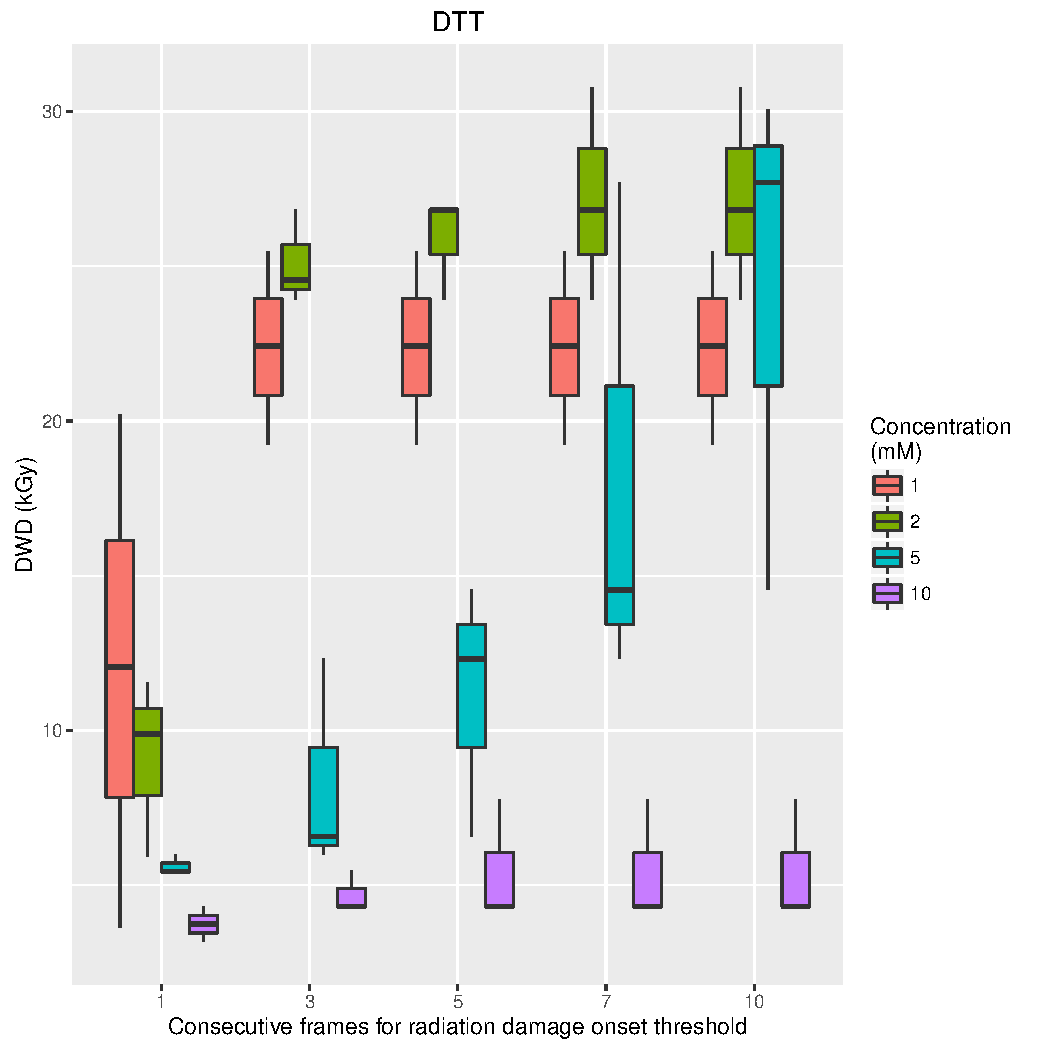
\includegraphics[width=0.8\textwidth]{figures/saxs/DTT_Num_consec_fr_comp.pdf}
    \caption{Dose at which significant radiation damage is determined to have occurred for different values of $m$ for DTT.}
    \label{fig:Num consec frames - DTT}
\end{figure}

\subsubsection{Pairwise comparisons with all frames}
\label{subs:Pairwise comparisons with all frames}
One assumption that is made in the merging analysis is that because the first frame suffers the least amount of dose, all subsequent frames should be compared to the first frame.
However if instead frames were compared to a different `reference frame' would the threshold be different?
Figure~\ref{fig:First n diff frames - DTT} answers this question.
Along the $y$-axis are the frames which would be considered as the merging limit if the corresponding frame on the $x$-axis was chosen as the `reference frame'.
It can be seen that the radiation threshold value obtained using the \textit{CorMap} metric is highly dependent on the reference frame.
This will greatly affect the conclusions that would be drawn from the analysis.
For example consider the first experimental run of GI sample with DTT added at $10\ mM$ concentration.
If the reference frame is 1, as is the case for the main analysis, then the frame at which radiation damage is considered as significant is frame 8 (DWD = $2.24\ KGy$).
However if the reference frame was 7 then the threshold frame would be 57 (DWD = $15.93\ kGy$).
This value is closer to the value obtained from the \textit{BsxCuBE} metric for that run (DWD = $22.92\ kGy$).
\begin{figure}
    \centering
    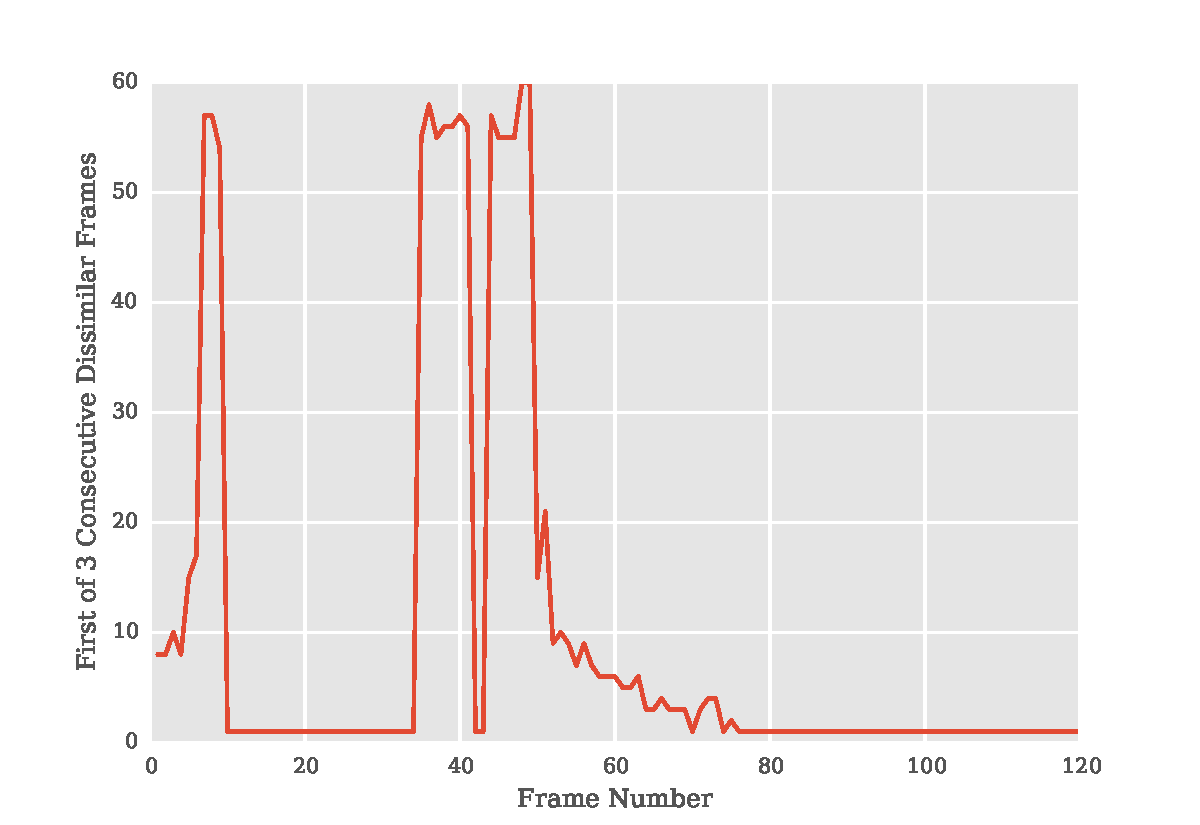
\includegraphics[width=0.8\textwidth]{figures/saxs/dtt_first_n_plot.pdf}
    \caption{Radiation damage threshold value against reference frame for $m = 3$.}
    \label{fig:First n diff frames - DTT}
\end{figure}

The fact that performing the pairwise comparisons with different reference frames gives different results suggests that more information can be gained by analysing the results from all possible pairwise comparisons.
Figure~\ref{fig:heatmap - DTT} is a heat map showing the results from all possible pairwise frame comparisons.
The first row shows the results that were obtained using frame 1 as the reference frame and it is evident that at frame 8 the \textit{CorMap} metric highlights that the frames become dissimilar.
However there is a huge square region of similar frames in the top left of the map suggesting that the best results may be obtained by merging the frames from the larger region which doesn't necessarily include the first frame.
The structure of this map could suggest that there are very quick changes occurring in the sample until a relatively stable molecular conformation is reached.
Perhaps if could be that merging frames from these different regions may result in data to suggest the molecules are in slightly different states.
\begin{figure}
    \centering
    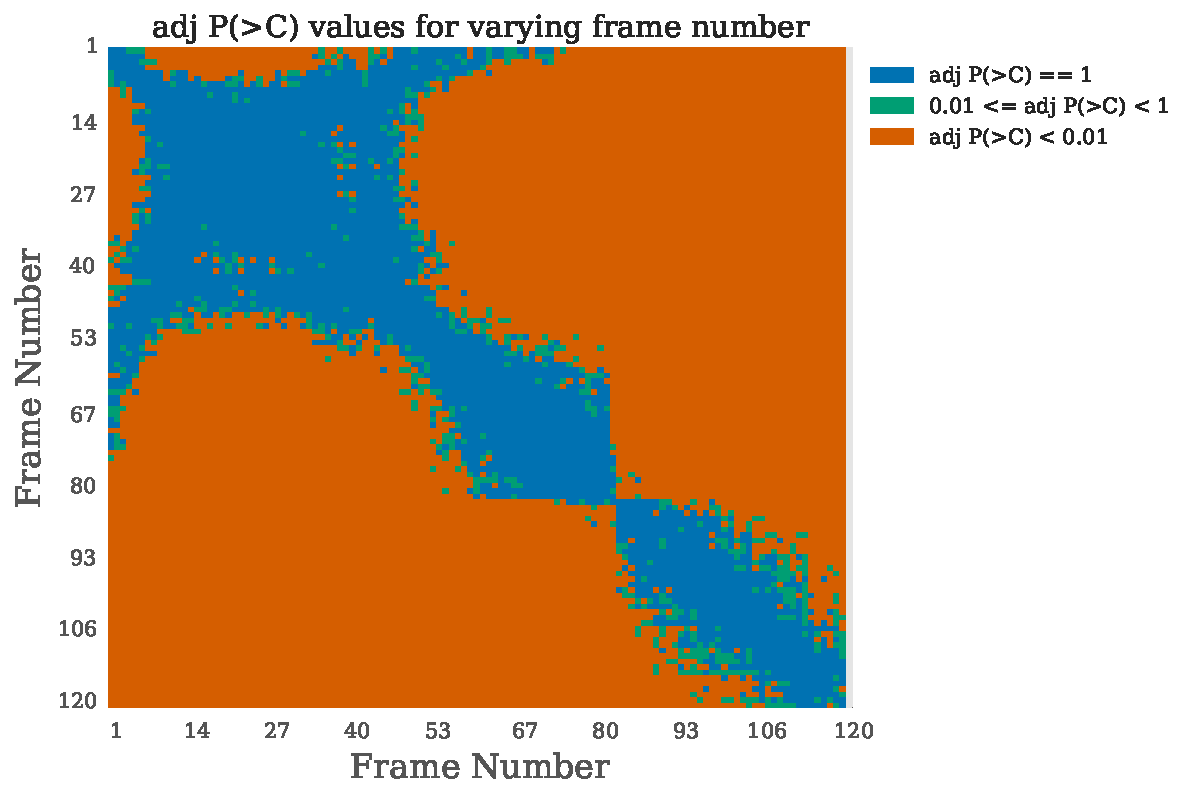
\includegraphics[width=0.8\textwidth]{figures/saxs/dtt_heatmap.pdf}
    \caption{heat map of all possible pairwise frame comparisons for the first GI sample run with $10\ mM$ concentration DTT added. The $y$-axis represents the reference frame to which all other frames on the $x$-axis are compared. Blue - $P_{adj}(>C) = 1$. Teal - $0.01 \le P_{adj}(>C) < 1 $. Orange - $P_{adj}(>C) < 0.01$.}
    \label{fig:heatmap - DTT}
\end{figure}

\subsubsection{Using dose value and frame number as damage thresholds}
\label{subs:Using dose value and frame number as damage thresholds}
Using the dose as the metric to evaluate the efficacy of the different radioprotectants means that the results are normalised for the energy absorption from the compounds. It is sensible to ask whether this normalisation changes the conclusions that would be drawn if the frame number alone was used as the threshold metric.
Figure~\ref{fig:SAXS dose vs frame} shows the results for the $1\ mM$ and the $10\ mM$ concentrations of radioprotectants with dose value and frame number as the damage thresholds.
For the more radiation tolerant samples there is not much difference in using either the dose or the frame number.
However for the less efficient radioprotectants (sucrose, TEMPO and trehalose) there is a significant difference.
If the frame number is used (Figures \ref{fig:SAXS frame- 1mM}, \ref{fig:SAXS frame- 10mM}) the order of the relative efficacies of those radioprotectants is not too obvious.
However if the dose value is used instead (Figures \ref{fig:SAXS dose- 1mM}, \ref{fig:SAXS dose- 10mM}) then the order becomes much clearer, particularly at $1\ mM$ concentration.
The spread of the threshold values for those compounds is also smaller using dose instead of frame number for the $10\ mM$ concentration.
\begin{figure}
    \centering
    \begin{subfigure}[b]{0.45\textwidth}
            \centering
            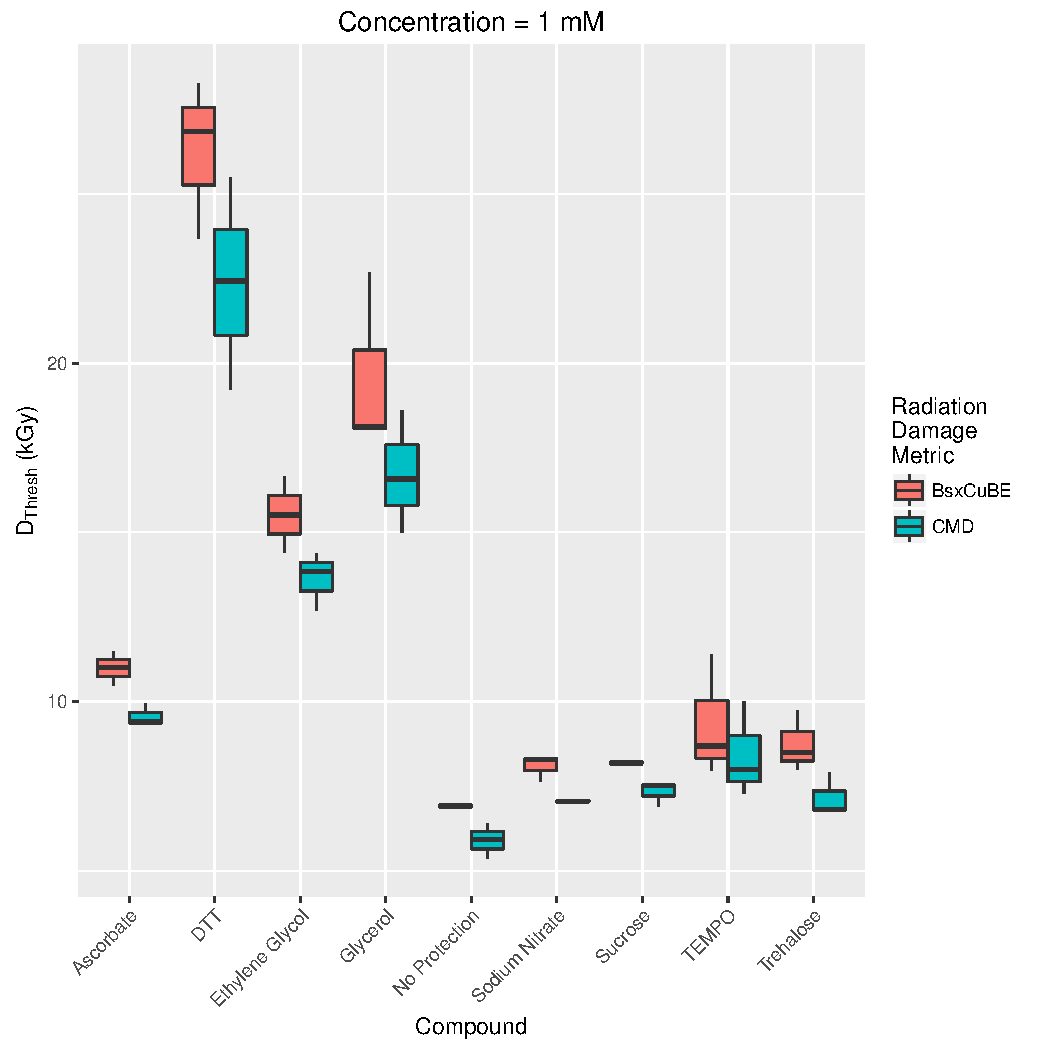
\includegraphics[width=\textwidth]{figures/saxs/Conc_1_dose.pdf}
            \caption{}
            \label{fig:SAXS dose- 1mM}
    \end{subfigure}
    \qquad
    \begin{subfigure}[b]{0.45\textwidth}
            \centering
            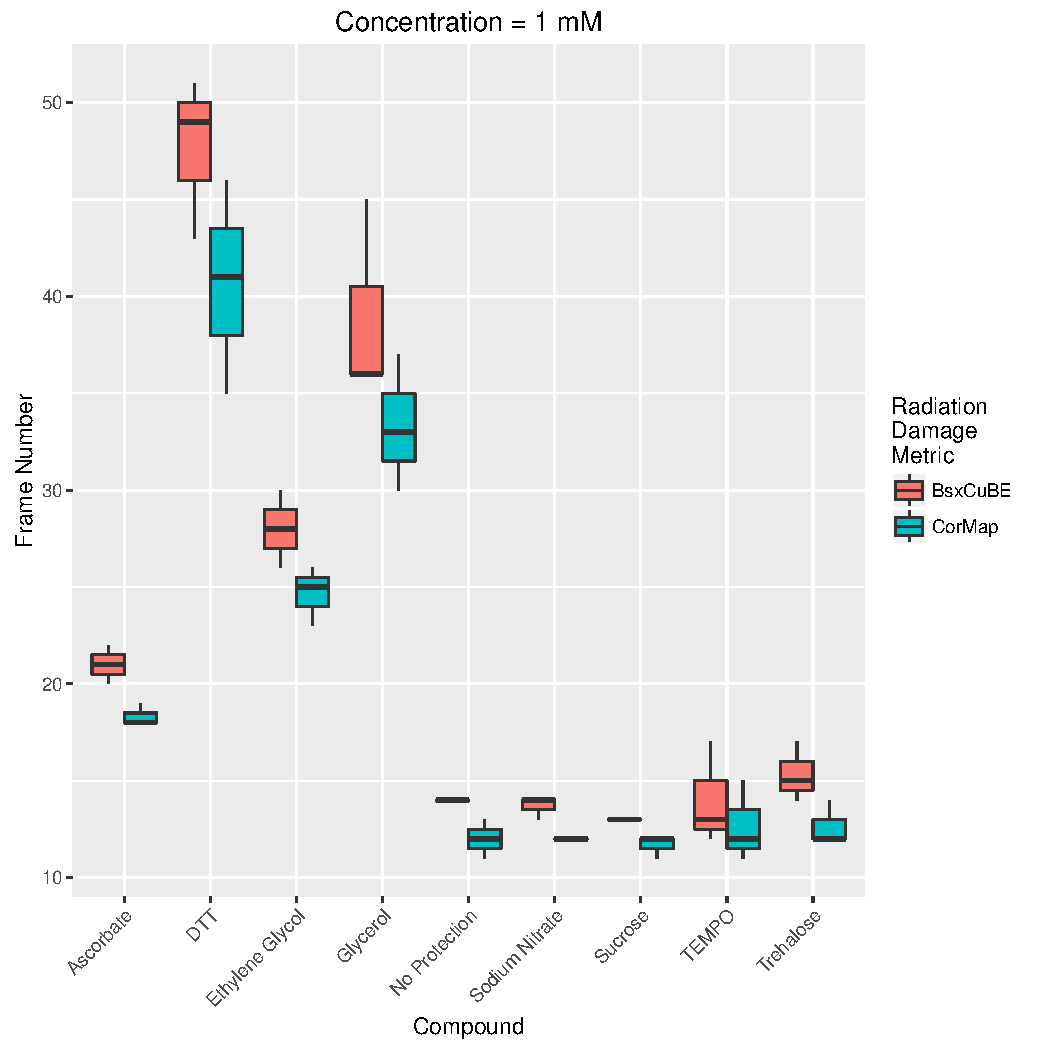
\includegraphics[width=\textwidth]{figures/saxs/Conc_1_frame_num.pdf}
            \caption{}
            \label{fig:SAXS frame- 1mM}
    \end{subfigure}
    \\
    \begin{subfigure}[b]{0.45\textwidth}
            \centering
            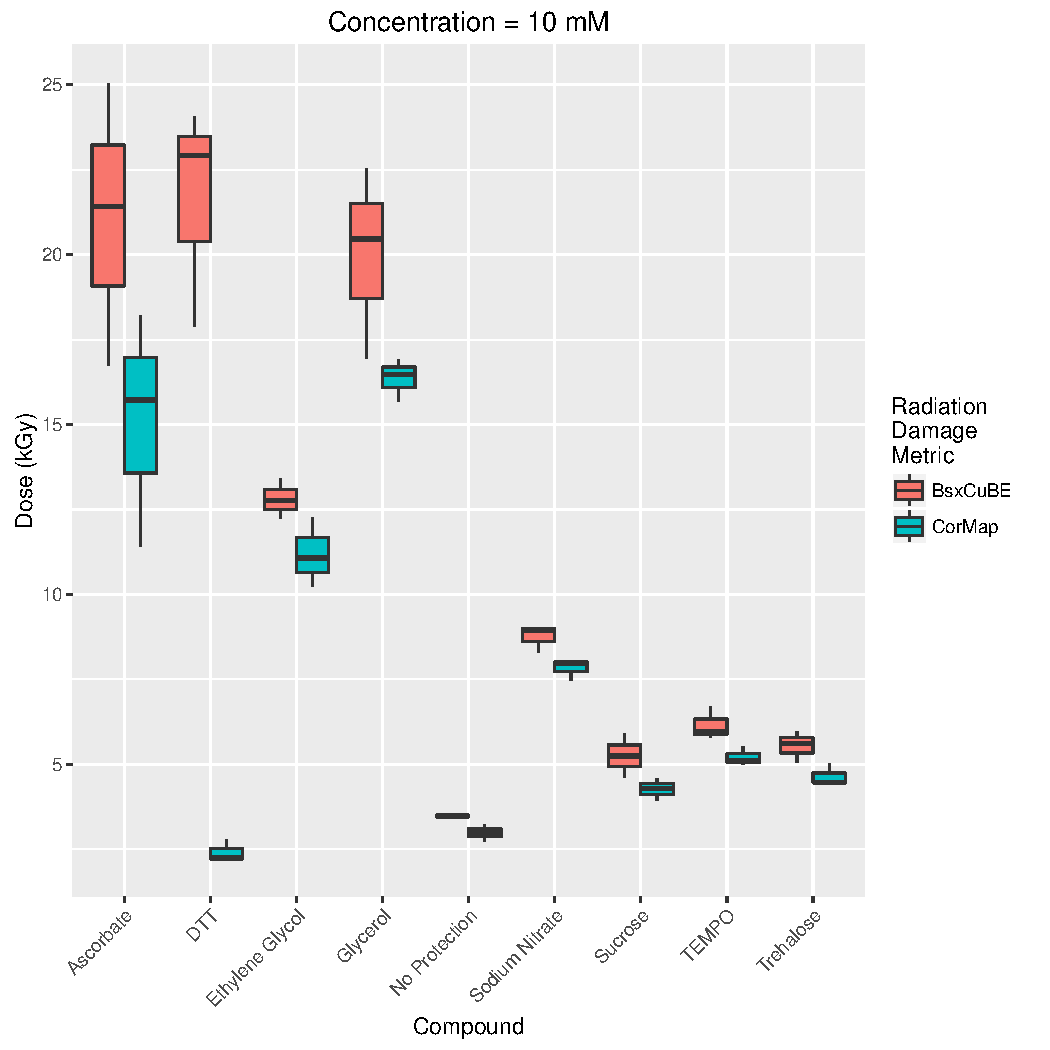
\includegraphics[width=\textwidth]{figures/saxs/Conc_10_dose.pdf}
            \caption{}
            \label{fig:SAXS dose- 10mM}
    \end{subfigure}
    \qquad
    \begin{subfigure}[b]{0.45\textwidth}
            \centering
            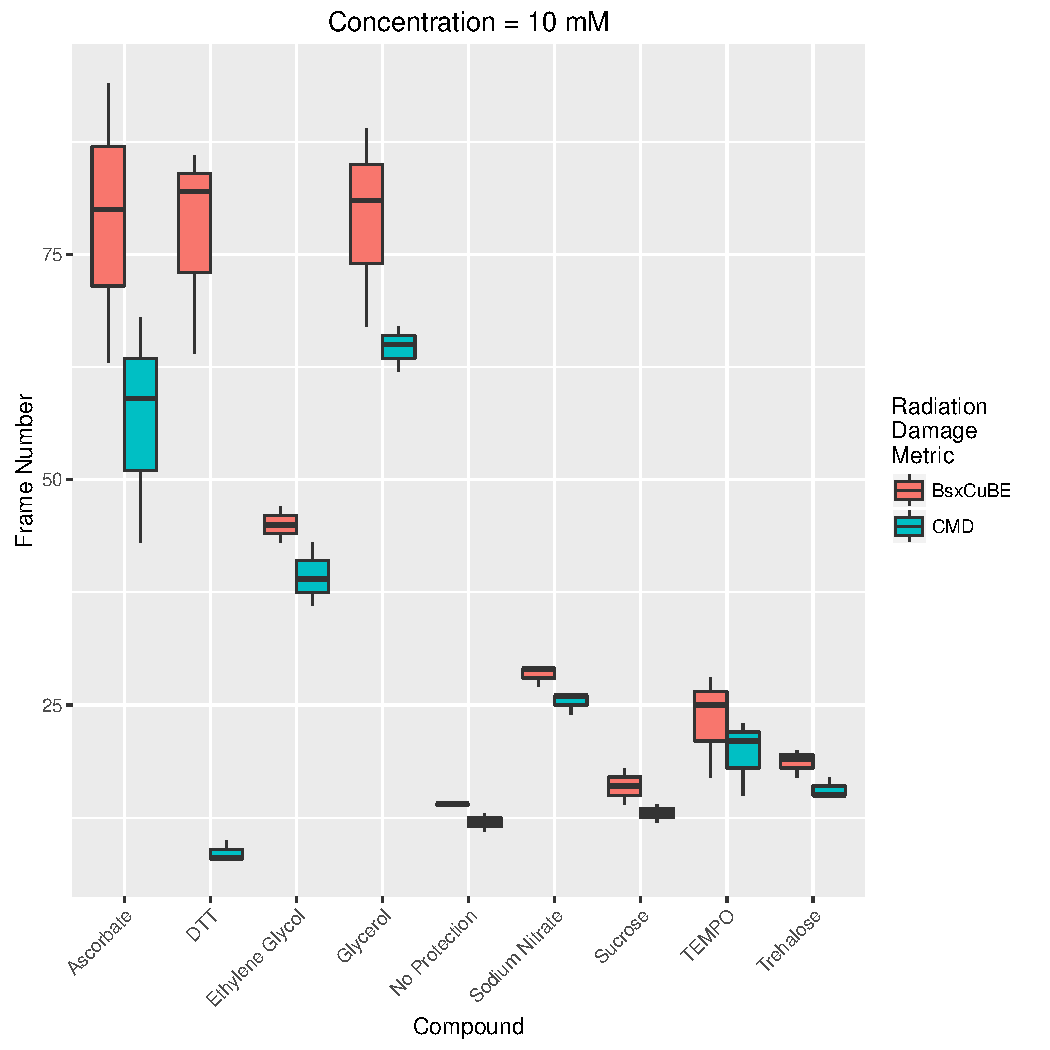
\includegraphics[width=\textwidth]{figures/saxs/Conc_10_frame_num.pdf}
            \caption{}
            \label{fig:SAXS frame- 10mM}
    \end{subfigure}
    \caption{Value at which radiation damage is considered significant. Figures on the left correspond to the dose value whereas figures on the right correspond to the frame number. Each box plot is created from the threshold dose values for three different runs of the same radioprotectant compound for each concentration. Pink boxes correspond to the \textit{BsxCuBE} metric, blue boxes correspond to the \textit{CorMap} metric.}
    \label{fig:SAXS dose vs frame}
\end{figure}

\subsubsection{Concentration dependence}
\label{subs:Concentration dependence}
A metric, RD onset ratio, was developed to assess the change in radiation tolerance in the sample with the radioprotectant added compared to no protection.
This metric is defined as the ratio of the median threshold value with added radioprotectant to the median of the threshold value without radioprotectant added using the \textit{CorMap} metric.
Values below 1 correspond to a reduction in radiation tolerance whereas values above 1 show improved radiation tolerance.
This metric was calculated for each compound at each concentration and the results are plotted in Figure~\ref{fig:SAXS Ratio plot}.
Significant concentration dependence can be observed for several radioprotectants.
In particular, ascorbate, glycerol, and sodium nitrate all exhibit a strong positive concentration dependence i.e. the higher the concentration, the better the protection ability.
DTT exhibits the opposite behaviour.
At low concentrations DTT has the highest ratio but decreases at the higher concentrations.
Sucrose, TEMPO and Trehalose show a very small positive dependence but even at the highest concentration ($10\ mM$) the RD onset ratio is less than 2.
The RD onset ratio for Ethylene glycol decreases as the concentration increases from $1\ mM$ to $5\ mM$, but then there is a large increase at $10\ mM$.
\begin{figure}
    \centering
    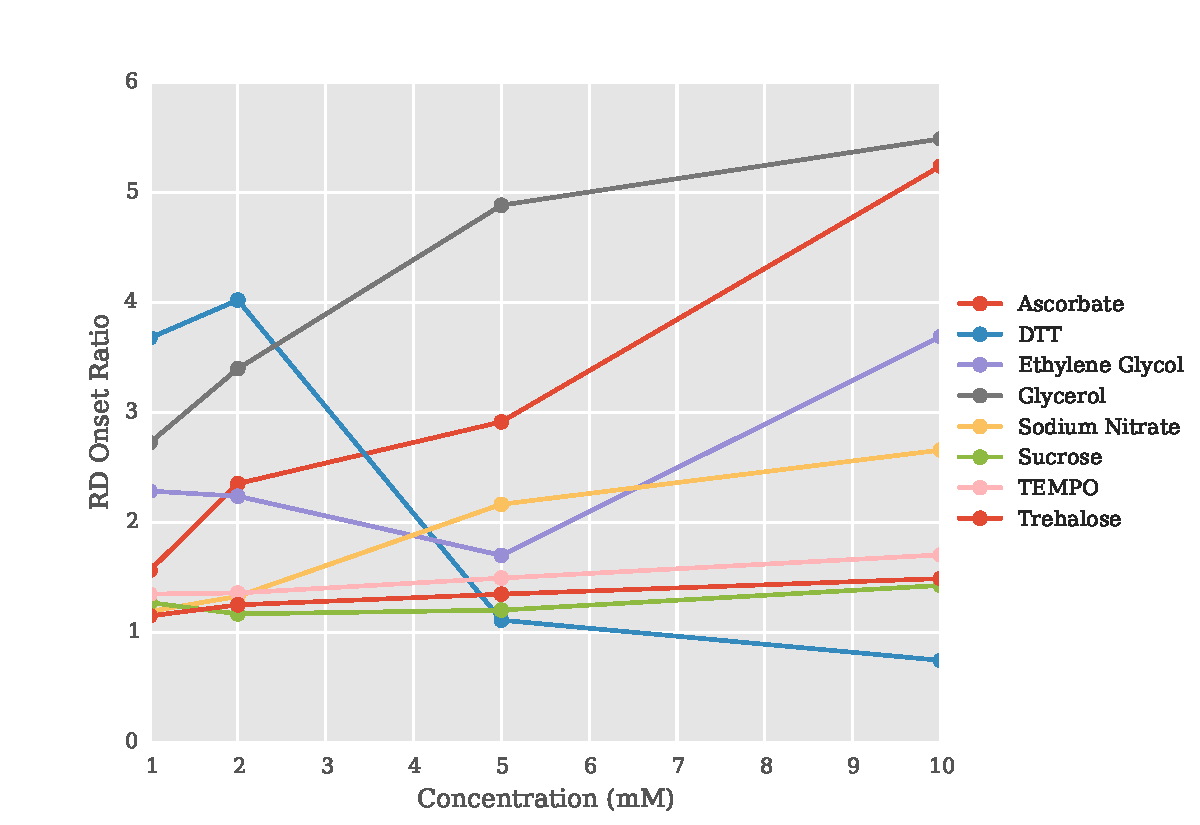
\includegraphics[width=0.8\textwidth]{figures/saxs/RatioPlots.pdf}
    \caption{RD onset ratio against concentration for the 8 radioprotectants.}
    \label{fig:SAXS Ratio plot}
\end{figure}

\subsubsection{Relative radioprotectant efficacy}
\label{subs:Relative radioprotectant efficacy}
Figure~\ref{fig:SAXS Ratio plot} shows that the most effective radioprotectant various depending on the concentration of the compound used in the sample.
Both the \textit{BsxCuBE} metric and the \textit{CorMap} metric agree that at low concentrations ($1\ mM$ and $2\ mM$) DTT is the most effective scavenger to use.
However at higher concentrations these metrics disagree.
At $5\ mM$ and $10\ mM$ the \textit{BsxCuBE} metric suggests that the most effective radioprotectant is still DTT.
On the otherhand, the \textit{CorMap} metric suggests that the best metric to use is glycerol and that DTT is the least effective radioprotectant.
Although it has been shown that using a different reference frame to perform pairwise comparisons can result in different results with the \textit{CorMap} metric (Figures~\ref{fig:First n diff frames - DTT} and \ref{fig:heatmap - DTT}).

The \textit{CorMap} metric result disagrees with the results from experiment 1 where ethylene glycol was found to be the most effective radioprotectant at $5\ mM$. This could be because the experimental parameters were not as well characterised in the first experiment as opposed to the second.
